\documentclass[]{article}
\usepackage{caption,subcaption,graphicx,float,url,amsmath,amssymb}
\usepackage[hidelinks]{hyperref}
\usepackage[toc,acronym]{glossaries}
\setacronymstyle{long-short}
\usepackage{glossaries-extra}
\graphicspath{{figs/}} 
%opening
\title{
	Notes from Origins of Life\\
	Week 3: Chemical Commonalities
}
\author{Simon Crase}

\makeglossaries

\loadglsentries{glossary}

\renewcommand{\glstextformat}[1]{\textbf{\em #1}}

\begin{document}

\maketitle

\begin{abstract}
 	These are my notes from Week 1 of the \gls{gls:SFI} Origins of Life Course\cite{sfi2019}. The course aims to push the field of Origins of Life research forward by bringing new and synthetic thinking to the question of how life emerged from an abiotic world.\\
  	The content and images contained herein are the intellectual property of the Santa Fe Institute, with the exception of any errors in transcription, which are my own.
  	These notes are distributed in the hope that they will be useful,
  	but without and warranty; without even the implied warranty of
  	merchantability or fitness for a particular purpose. All feedback is welcome,
  	but I don't necessarily undertake to do anything with it.
\end{abstract}

\setcounter{tocdepth}{2}
\tableofcontents

\listoffigures

\section{Introduction}

This week is a more detailed look at biochemistry: biological information encoded in chemistry; the chemical processes that drive organization; and how life extracts energy from its environment.

\section{DNA as Information}
Lecturer: Michael Lachmann, \gls{gls:SFI}

In this section we see that DN is noisier than we think. Error rate $10^{-10}$ errors per (replication*bas pair)
\subsection{DNA as Information - I}



\begin{figure}[H]
	\caption{The 4 Nucleotides in DNA}\label{fig:Nucleotides} 
	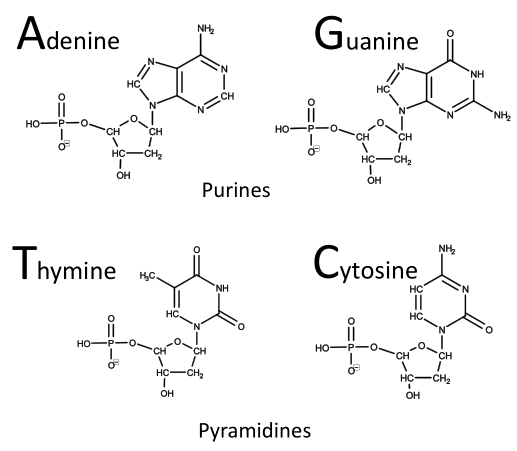
\includegraphics[width=0.9\textwidth]{Nucleotides}
\end{figure}

\begin{figure}[H]
	\caption{A closer look at one Nucleotide, Adenine}\label{fig:NucleotideAdenine} 
	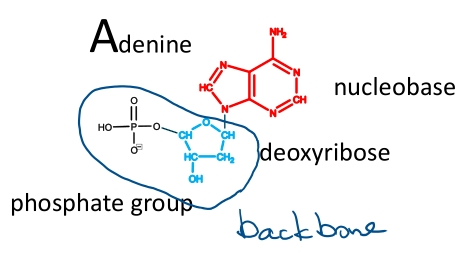
\includegraphics[width=0.9\textwidth]{NucleotideAdenine}
\end{figure}

\begin{figure}[H]
	\caption{The only chemical difference between DNA and RNA is the extra OH group in RNA, which makes the molecule more active. DNA is more stable. }\label{fig:NucleotideDNARNA} 
	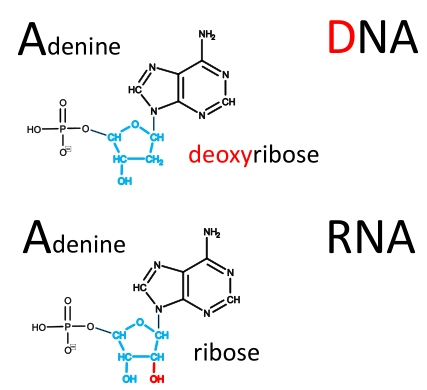
\includegraphics[width=0.9\textwidth]{NucleotideDNARNA}
\end{figure}

\begin{figure}[H]
	\caption{RNA used Uracil instead of Thymine. Note that Thymine is Uracil with an extra methyl group, hence the alternative name $5-methyluracil$. The $5$ comes from the numbering of carbon atoms--see \ref{fig:NucleotidesCounting} }\label{fig:NucleotideDNARNAThymineUracil} 
	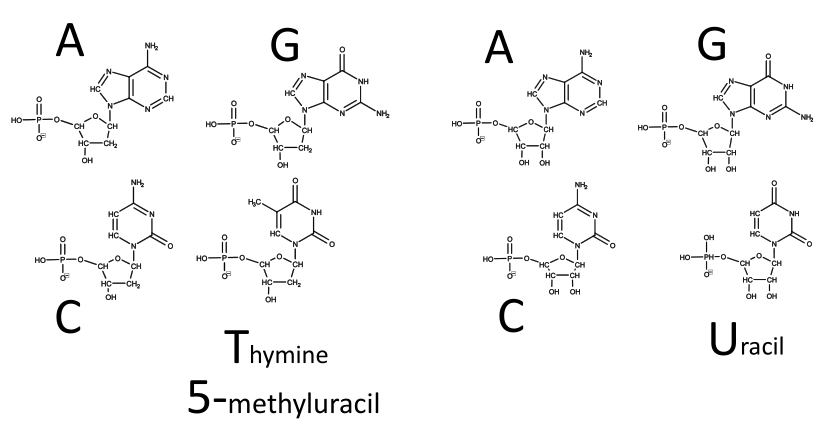
\includegraphics[width=0.9\textwidth]{NucleotideDNARNAThymineUracil}
\end{figure}

\begin{figure}[H]
	\caption{Numbering of carbon atoms in purines and pyrimidines. }\label{fig:NucleotidesCounting} 
	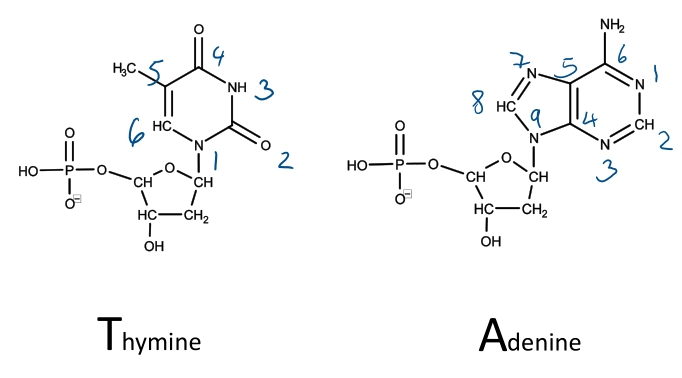
\includegraphics[width=0.9\textwidth]{NucleotidesCounting}
\end{figure}

\begin{figure}[H]
	\caption{A selection of 12 modified bases}\label{fig:ModifiedBases} 
	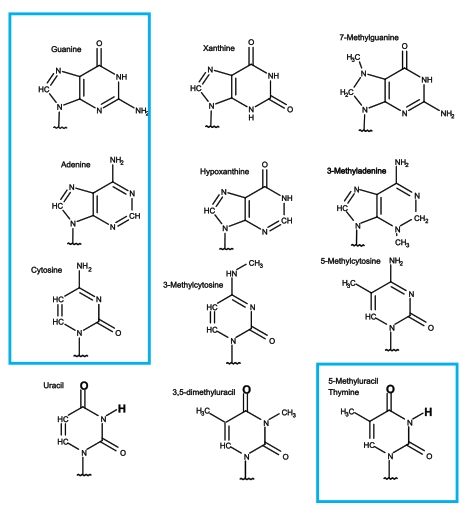
\includegraphics[width=0.9\textwidth]{ModifiedBases}
\end{figure}

\gls{gls:deamination}

\begin{figure}[H]
	\caption{44 Modified DNA nucleobases have actually been observed.\cite{sood2019dnamod},\cite{sood2019dnamod_website} } \label{fig:ModifiedDNA_Nucleobases} 
	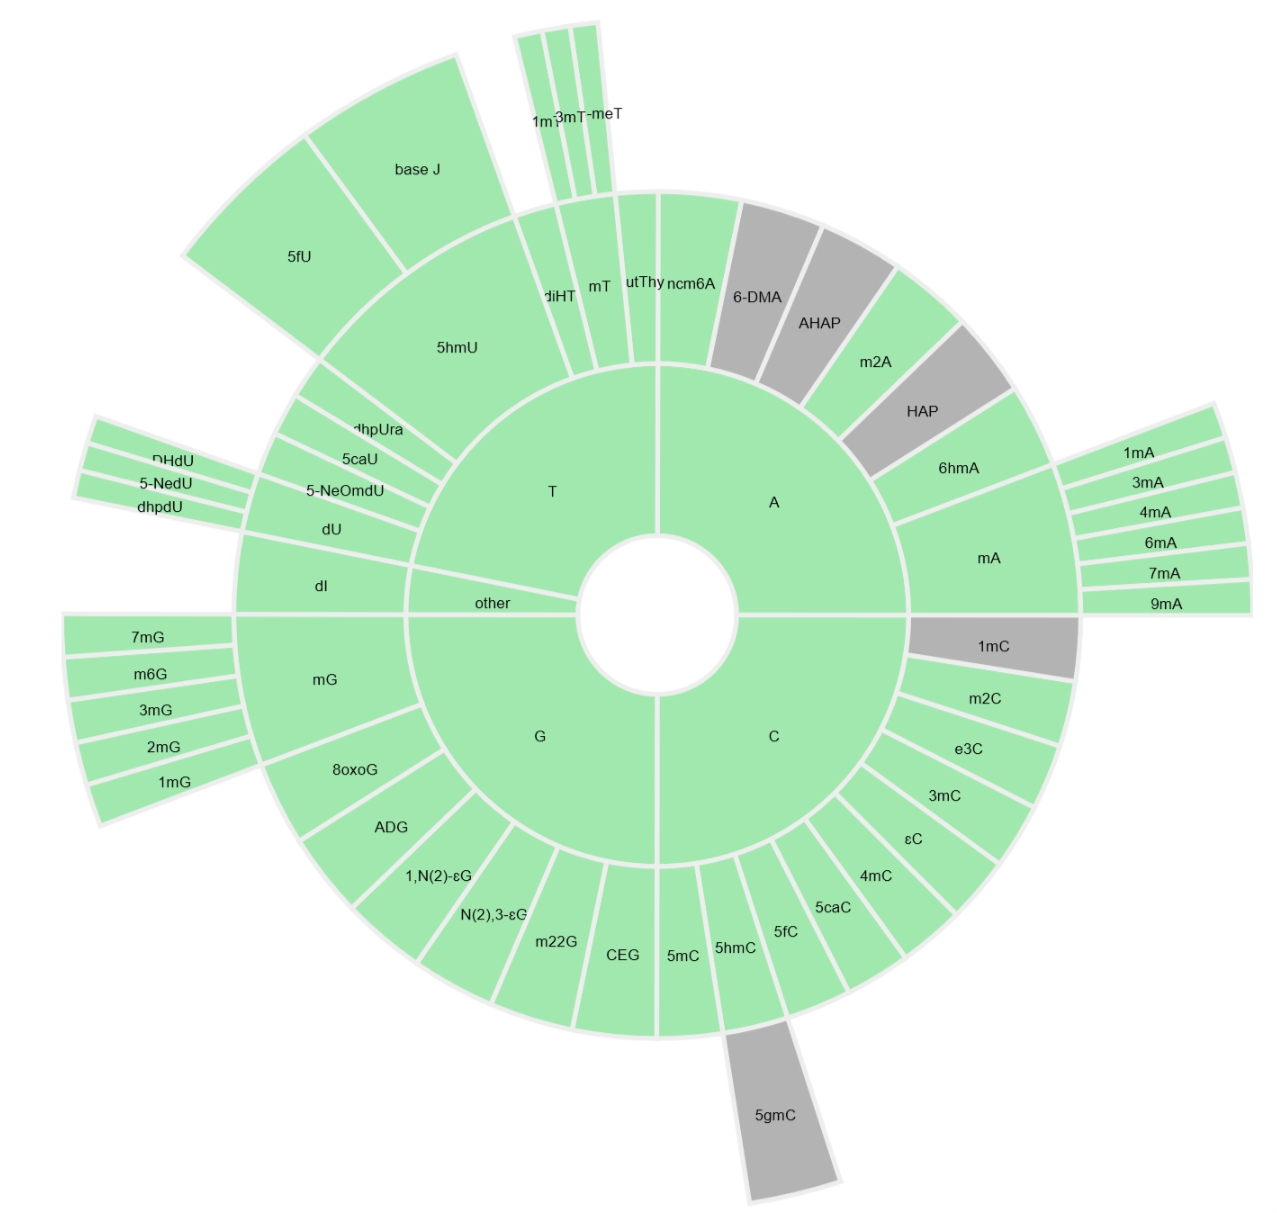
\includegraphics[width=0.9\textwidth]{ModifiedDNA_Nucleobases}
\end{figure}

The are a couple of bacteriophages, PBS1 and PBS2, that contain Uracil instead of thymine in their DNA\cite{hemphill1975bacteriophages}. Either the thymine has been replaced, or these phages are more primitive, and never used thymine.

When people talk about methylation of DNA, they usually mean $5-methylcytosine$, Figure \ref{fig:5methylcytosine}, even though there are many other ways to do it
\begin{figure}[H]
	\caption{$5-methylcytosine$ } \label{fig:5methylcytosine} 
	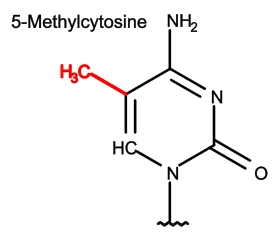
\includegraphics[width=0.9\textwidth]{5-methylcytosine}
\end{figure}

Methylation tends to occur when C is followed by G. The methylated versions are replicated us unmethylated C, but there is an enzyme, \gls{gls:DNAmethyltransferase}, which performs methylation, as shown in Figure \ref{fig:5-methylcytosine-in-action}. This can carry epigenetic changes across cell divisions, and sometimes across generations. This is important as it means that a lever cell can "remember" that is comes from a liver cell.
\begin{figure}[H]
	\caption{Methylation tends to occur when C is followed by G } \label{fig:5-methylcytosine-in-action} 
	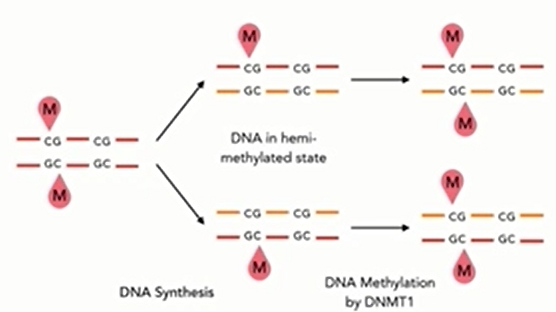
\includegraphics[width=0.9\textwidth]{5-methylcytosine-in-action}
\end{figure}

6-Methyladenine is also important--Figure \ref{fig:6-Methyladenine}-- in bacteria, where it carries information regarding the old strand versus the new. The methylation isn't very fast, so it can distinguish old from new. Section \ref{section:DNAasInfo2} shows how this is useful for repair.

\begin{figure}[H]
	\caption{6-Methyladenine is also important (palindromic sequence)} \label{fig:6-Methyladenine} 
	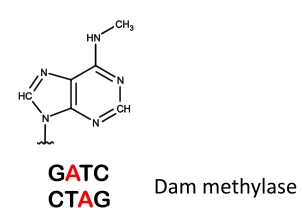
\includegraphics[width=0.9\textwidth]{6-Methyladenine}
\end{figure}

\begin{figure}[H]
	\caption{ModifiedRNAdatabase \cite{agriss2019RNA}} \label{fig:ModifiedRNAdatabase} 
	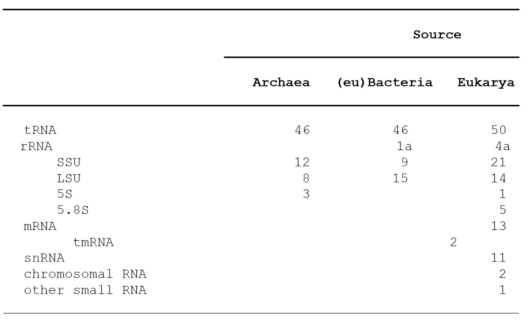
\includegraphics[width=0.9\textwidth]{ModifiedRNAdatabase}
\end{figure}

\textbf{Summary}

\begin{itemize}
	\item 44 DNA mod
	\item 112 RNA mod
	\item Many survive 	replication
	\item Some are replicated themselves
	\item Functional: 5mC, 6mA, 5hmC, RNA \&more
	\item Generated:
\begin{itemize}
	\item Enzyme activity
	\item Damage
	\item Misincorporation
\end{itemize}
\end{itemize}

Where did the modifications come from? They could be fairly new, and we use them in various ways; or maybe they tell us something about the origin of DNA. Maybe there are many enzymes left over from before we had sophisticated machinery for DNA replication.

\subsection{DNA as Information - II}\label{section:DNAasInfo2}

\cite{kunkel2004dna}

\section{Water as a Driving Force for Organization}

\cite{ball2017water}

\section{Kinetic vs. Thermodynamics – Assembly Constraints}

\cite{pross2017and},\cite{semenov2016autocatalytic},\cite{pross2008can}, \cite{dee2016comparing},\cite{pross2005emergence}

\section{Chemical Configurations: Proteins and DNA}

\section{Early Metabolisms}
\cite{bar2011survey}, \cite{fuchs2011alternative}, \cite{weiss2016physiology}

\section{Energy Harvesting}

\cite{simon2008organisation}

\section{Systematics and Limits of Metabolic Rates}

% end of text 

% glossary
\printglossaries

% bibliography goes here
 
\bibliographystyle{unsrt}
\addcontentsline{toc}{section}{Bibliography}
\bibliography{origins}

\end{document}
